\documentclass[bwprint]{gmcmthesis}
\usepackage{amsmath}
\usepackage{multirow}
\usepackage{threeparttable}
\usepackage{pifont}
\numberwithin{figure}{section}
\renewcommand{\thefigure}{\arabic{section}-\arabic{figure}} 
\newcommand{\upcite}[1]{\textsuperscript{\textsuperscript{\cite{#1}}}}
% \documentclass[withoutpreface,bwprint]{cumcmthesis}
% 去掉封面与编号页

\title{中国研究生数学建模竞赛论文标题}
\baominghao{No.21104870023} %参赛队号
\schoolname{华中科技大学}%学校名称
\membera{张智璐} %队员A
\memberb{钱以骞} %队员B
\memberc{周鑫宜} %队员C
\begin{document}
 \maketitle
 \begin{abstract}
第一段:针对自己选择的题目,说明自己用了什么方法来解决的(这类题属于哪种典型的问题),其中利用了哪些关键的算法,再说出自己的所建模型的创新点。没有创新点,也可以说自己所建的模型相比较于其它的是一个很好的方案。

第二段:问题一中,针对具体问题,进行分析和求解,几句话介绍自己是怎么解决的,有数字结果的也可以直接贴结果。

第三段:问题二中,类比于第二段。

第四段:问题三中,类比于第三段。

第五段:问题四中,类比于第四段。

第六段:如果有问题五,类比于第五段,没有就结束,也可以写一下团队的想法。

随便加点东西






\keywords{针对具体的问题列一到两个关键字\quad  建模算法列出\quad }
\end{abstract}

%\pagestyle{plain}

%目录
\tableofcontents

\section{问题重述}
\subsection{问题背景}
环境空气污染能够对人类、动植物及产生较大的影响和危害。建立空气质量预报模型,提前预报大气污染状况能够支撑政府制定防治策略,提醒公众提前防范,减少自身暴露,减轻污染。

WRF-CMAQ模拟体系(以下简称WRF-CMAQ模型)是在 “一个大气” 理论的指导下,以WRF中尺度数值天气预报系统为依托,充分考虑了大气污染过程中水平传输、垂直传输、扩散过程、源排放、化学反应和去除过程等对污染物浓度的影响,将复杂空气污染状况进行综合处理\upcite{ref1}。WRF和CMAQ的结构如图\ref{fig1-1}和图\ref{fig1-2}所示。
\begin{figure}[!h]
	\centering
	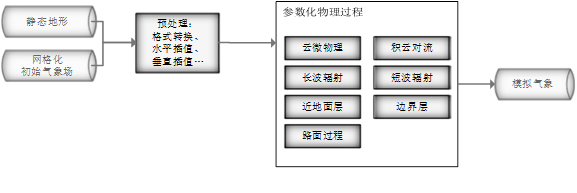
\includegraphics[width=.7\textwidth]{figures//fig1-1.png}
	\caption{中尺度数值天气预报系统WRF结构\upcite{ref2}}
	\label{fig1-1}
\end{figure}
\begin{figure}[!h]
	\centering
	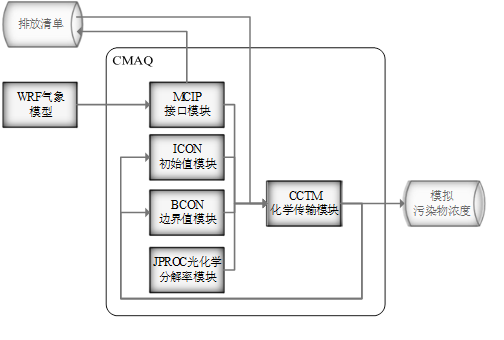
\includegraphics[width=.7\textwidth]{figures//fig1-2.png}
	\caption{空气质量预测与评估系统CMAQ结构\upcite{ref3}}
	\label{fig1-2}
\end{figure}

CMAQ是一种三维欧拉大气化学与传输模拟系统,经由对污染物变化过程的模拟得到具体时间点或时间段的预报结果,但由于模拟的气象场和排放清单的不确定性,同时还存在包括臭氧在内生成机理不完全明晰的污染物的存在,WRF-CMAQ预报模型的结果并不理想。为提高预报准确性,一种可行办法是在WRF-CMAQ等一次模型模拟结果的基础上,结合更多的数据源进行二次建模。二次模型与WRF-CMAQ模型关系如图\ref{fig1-3}所示。其中,由于气象条件对空气质量影响很大(例如湿度降低有利于臭氧的生成),且污染物浓度实测数据的变化情况对空气质量预报具有一定参考价值,因此实测数据源参考空气质量监测点获得的气象数据。
\begin{figure}[!h]
	\centering
	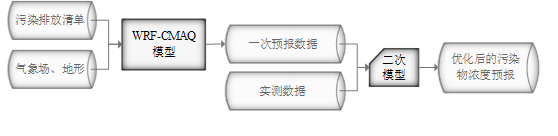
\includegraphics[width=.7\textwidth]{figures//fig1-3.png}
	\caption{空气质量预测与评估系统CMAQ结构}
	\label{fig1-3}
\end{figure}

\subsection{问题提出}
\textbf{问题1}使用附件1数据,计算监测点A从2020年8月25日到8月28日每天实测的AQI和首要污染物。并将结果按照表\ref{tab:table1-1}格式放于正文中
\begin{table}[h!]
	\caption{AQI计算结果表}\label{tab:table1-1}
	\begin{center}
		\begin{tabular}{|c|c|c|c|}
			\hline
			\multirow{2}{*}{检测日期}&\multirow{2}{*}{地点}&\multicolumn{2}{|c|}{AQI计算} \\
			\cline{3-4}
			& &AQI&首要污染物\\
			\hline
			2020/8/25&监测点A&&\\
			\hline
			2020/8/26&监测点A&&\\
			\hline
			2020/8/27&监测点A&&\\
			\hline
			2020/8/28&监测点A&&\\
			\hline
		\end{tabular}
	\end{center}
\end{table}

\textbf{问题2}使用附件1中的数据,根据对污染物浓度的影响程度,对气象条件进行合理分类,并阐述各类气象条件的特征。


\textbf{问题3}使用附件1和2的数据,建立适用3个监测点(忽略彼此影响)的二次预报数学模型,预测未来3天6种污染物浓度,要求预测结果AQI最大相对误差尽量小,首要污染物预测准确度尽量高。并用该模型预测ABC的2021年7月13到7月15的污染物浓度,计算AQI和首要污染物。将结果按照表\ref{tab:table1-2}的格式放于正文中
\begin{table}[h!]
	\caption{AQI计算结果表}\label{tab:table1-2}
	\begin{center}
	\resizebox{.95\columnwidth}{!}{
		\begin{tabular}{|c|c|c|c|c|c|c|c|c|c|}
			\hline
			\multirow{2}{*}{预报日期}&\multirow{2}{*}{地点}&\multicolumn{8}{|c|}{二次模型日值预测} \\
			\cline{3-10}
			& &SO2(μg/m³)&NO2(μg/m³)&PM10(μg/m³)&PM2.5(μg/m³)&O3最大八小时滑动平均(μg/m³)&CO(mg/m³)&AQI&首要污染物\\
			\hline
			2020/7/13&监测点A&&&&&&&&\\
			\hline
			2020/7/14&监测点A&&&&&&&&\\
			\hline
			2020/7/15&监测点A&&&&&&&&\\
			\hline
		\end{tabular}
	}
	\end{center}
\end{table}


\textbf{问题4}使用附件1和3数据建立区域协同预报模型,包含A,A1,A2,A3四个监测点。要求预测结果AQI最大相对误差尽量小,首要污染物预测准确度尽量高。使用该协同预报模型预测监测点A、A1、A2、A3在2021年7月13日至7月15日的污染物浓度,计算AQI和首要污染物。将结果按照表\ref{tab:table1-2}的格式放于正文中。并讨论协同预报模型是否能提升准确度。

\section{背景阐述、模型合理假设以及符号说明}
\subsection{背景阐述}
在该问题中,涉及到很多与不同领域有关的背景知识,在本节中对部分背景信息进行简单的阐述。
以下分别介绍每种气象条件因素的定义:
\begin{itemize}
	\item 温度是表示物体冷热程度的物理量,微观上来讲是物体分子热运动的剧烈程度。温度只能通过物体随温度变化的某些特性来间接测量,而用来量度物体温度数值的标尺叫温标。在本文中,使用的温标为摄氏温标(°C)。本文中,将该变量简称为T。
	\item 比湿是空气中的水汽质量在混合空气中的质量占比,即
	$$\rm H≡\frac{m_v}{m_v+m_a}$$
	式中,H为比湿,无量纲;$\rm m_v$为空气中的水汽质量,单位:kg;$\rm m_a$为干空气质量,单位:kg。在本文中将该变量简称为H。
	\item 气压是作用在单位面积上的大气压力,即在数值上等于单位面积上向上延伸到大气上界的垂直空气柱所受到的重力。在本文中,使用单位为MPa, 1MPa = 1000000pa。将该变量简称为P。
	\item 风速是指空气相对于地球某一固定地点的运动速率,本文中使用的单位是m/s,1m/s=3.6km/h。本文将该变量简称为WS。
	\item 风向是指风的来向,本题用角度表示。定义自正北方向至监测点的风向为0°风向,以顺时针旋转角(单位:°)为正值记录风向。例如,风自正东方向至监测点时,记录此时段风向为90°。本文将该变量简称为WD。
\end{itemize}
\subsection{模型合理假设}
a.假设本题涉及到的所有大气科学相关变量(气象条件或是污染物浓度等)在自然界都是连续变量

b.在一段连续时间内,由工业、生活等人类日常行为产生的污染物排放浓度大致不变

c.
\subsection{符号说明}

\section{问题的分析}
\subsection{问题一:通过给定污染物数据计算当日的AQI指数}
\subsubsection{AQI指数计算方式与相关背景}
AQI即为空气质量指数,该数据可用于判别空气质量等级。AQI的计算方式如下:
首先需得到各项污染物的空气质量分指数(IAQI),其计算公式如公式(1)所示:
\begin{equation}
	\rm IAQI_P = \frac{IAQI_{Hi}-IAQI_{Lo}}{BP_{Hi}-BP_{Lo}}*(C_P-BP_{Lo})+IAQI_{Lo}
\end{equation}
式中各符号的含义如下:
\begin{itemize}
	\item $\rm IAQI_P$表示污染物P的空气质量分指数,结果进位取整数
	\item $\rm C_P$表示污染物P的质量浓度值
	\item $\rm BP_{Hi}, BP_{Lo}$表示与$\rm C_P$相近的污染物浓度限值的高位值与低位值
	\item $\rm IAQI_{Hi}, IAQI_{Lo}$表示与$\rm BP_{Hi},BP_{Lo}$对应的空气质量分指数
\end{itemize}

各项污染物项目浓度限值及对应的空气质量分指数级别见表\ref{tab:table4-1}:
\begin{table}[h!]
\caption{空气质量分指数(IAQI)及对应的污染物项目浓度限值}\label{tab:table4-1}
\begin{center}
\begin{threeparttable}
\resizebox{.95\columnwidth}{!}{
\begin{tabular}{|c|c|c|c|c|c|c|c|c|c|c|}
	\hline
	序号&指数或污染物项目&\multicolumn{8}{|c|}{空气质量分指数及对应污染物浓度限值}&单位 \\
	\hline
	0&空气质量分指数(IAQI)&0&50&100&150&200&300&400&500&-\\
	\hline
	1&一氧化碳(CO)24小时平均&0&2&4&14&24&36&48&60&$\rm mg∕m^3$\\
	\hline
	2&二氧化硫(SO2)24小时平均&0&50&150&475&800&1600&2100&2620&\multirow{5}{*}{$\rm μg∕m^3$} \\
	\cline{1-10}
	3&二氧化氮(NO2)24小时平均&0&40&80&180&280&565&750&940& \\
	\cline{1-10}
	4&臭氧(O3)最大8小时滑动平均&0&100&160&215&265&800&-&-& \\
	\cline{1-10}
	5&粒径小于等于10μm颗粒物
	(PM10)24小时平均&0&50&150&250&350&420&500&600& \\
	\cline{1-10}
	6&粒径小于等于2.5μm颗粒物
	(PM2.5)24小时平均&0&35&75&115&150&250&350&500& \\
	\hline
\end{tabular}
}
\begin{tablenotes}
	\footnotesize
	\item[1] 臭氧(O3)最大8小时滑动平均浓度值高于800 $\rm μg∕m^3$的,不再进行其空气质量分指数计算。
	\item[2] 其余污染物浓度高于IAQI=500对应限值时,不再进行其空气质量分指数计算
\end{tablenotes}
\end{threeparttable}      
\end{center}
\end{table}

空气质量指数(AQI)取各分指数中的最大值,即有
\begin{displaymath} 
	\rm AQI = max{IAQI_1,IAQI_2,...,IAQI_n}
\end{displaymath}
式中,$\rm IAQI_1,IAQI_2,IAQI_3,…,IAQI_n$为各污染物项目的分指数。在本题中,对于AQI的计算仅涉及表1提供的六种污染物,因此计算公式如公式(2)所示:
\begin{equation} 
	\rm AQI = max⁡{IAQI_{SO_2},IAQI_{NO_2},IAQI_{PM_10},IAQI_{PM_2.5},IAQI_{O_3},IAQI_CO}
\end{equation}
空气质量等级范围根据AQI数值划分,等级对应的AQI范围见表\ref{tab:table4-2}。
\begin{table}[h!]
	\caption{空气质量等级及对应空气质量指数(AQI)范围}\label{tab:table4-2}
	\begin{center}
		\begin{tabular}{|c|c|c|c|c|c|c|}
			\hline
			空气质量等级&优&良&轻度污染&中度污染&重度污染&严重污染 \\
			\hline
			空气质量指数(AQI)范围&[0,50]&[51,100]&[101,150]&[151,200]&[201,300]&[301,+∞) \\
			\hline
		\end{tabular}
	\end{center}
\end{table}

当AQI小于或等于50(即空气质量评价为“优”)时,称当天无首要污染物;
当AQI大于50时,IAQI最大的污染物为首要污染物。若IAQI最大的污染物为两项或两项以上时,并列为首要污染物
IAQI大于100的污染物为超标污染物。
则求解问题一需要根据附件1中提供的“监测点A逐日污染物浓度数据”表,通过上述方法计算监测点A从2020年8月25日到8月28日每天实测的AQI和首要污染物。
\subsubsection{快速求解AQI指数算法及对应结果}
求解AQI指数的过程非常简单,但是我们为了后期处理的方便性以及增强代码的可重用性,我们采用直接完全处理附件1中的“监测点A逐日污染物浓度数据”表的方式。在得到整个表的结果后,找出题目中的日期范围对应的结果。处理整个表格的流程图如图\ref{fig3-1}所示:
\begin{figure}[!h]
	\centering
	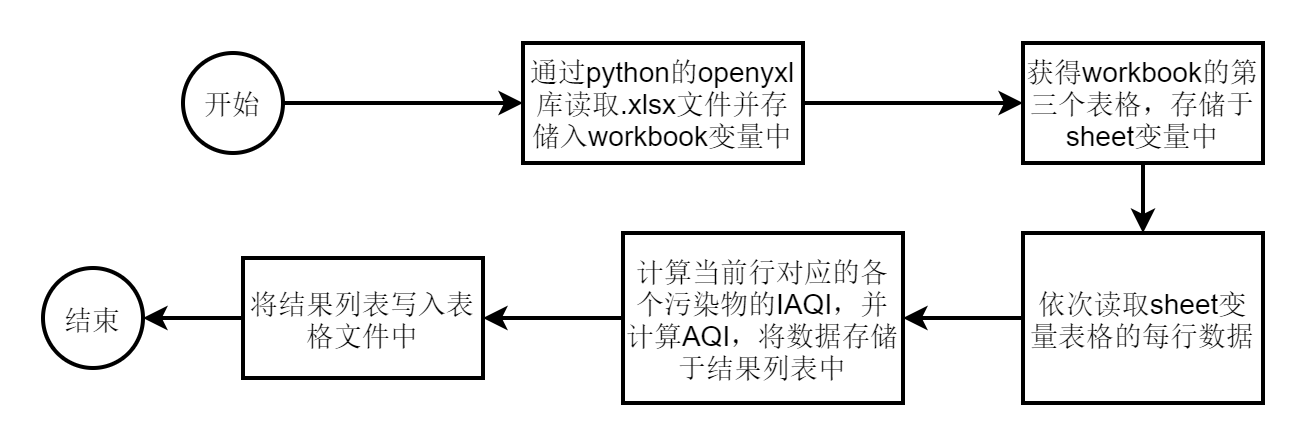
\includegraphics[width=.7\textwidth]{figures//fig3-1.png}
	\caption{完全处理“监测点A逐日污染物浓度数据”表流程图}
	\label{fig3-1}
\end{figure}

计算得到的结果如表\ref{tab:table4-3}所示
\begin{table}[h!]
	\caption{问题一AQI计算结果表}\label{tab:table4-3}
	\begin{center}
		\begin{tabular}{|c|c|c|c|}
			\hline
			\multirow{2}{*}{检测日期}&\multirow{2}{*}{地点}&\multicolumn{2}{|c|}{AQI计算} \\
			\cline{3-4}
			& &AQI&首要污染物\\
			\hline
			2020/8/25&监测点A&60&$\rm O_3$\\
			\hline
			2020/8/26&监测点A&46&无\\
			\hline
			2020/8/27&监测点A&109&$\rm O_3$\\
			\hline
			2020/8/28&监测点A&138&$\rm O_3$\\
			\hline
		\end{tabular}
	\end{center}
\end{table}

\subsection{问题二 根据对污染物浓度的影响程度,对气象条件进行分类}
\subsubsection{问题分析与数据预处理}
根据附件1中“监测点A逐小时污染物浓度与气象实测数据”表的数据,我们可以得到可能对污染物浓度产生影响的气象条件因素有5种:温度,比湿,气压,风速与风向。其具体定义

在污染物排放情况不变的条件下,某一地区的气象条件有利于污染物扩散或沉降时,该地区的AQI会下降,反之会上升。分析出,在不同气象条件下的AQI指数可以很好地反应气象条件对污染物浓度的影响。与此同时,也要分别分析6种污染物(CO,NO2,SO2,O3,PM10,PM2.5)在不同气象条件下的浓度变化情况。因此,首先计算AQI变量与各个污染物变量的相关性,然后通过主客观集成赋权法得到6种污染物浓度分别对我们最终定义的污染物浓度变量(称为AP)的影响权重。再通过各个污染物成为首要污染物的比例,对影响权重进行修正。最后建模得到气象因素对AP的影响,我们可以将气象条件因素分为三类:有较为显著的单向影响因素,有较为显著的双向影响因素,无显著影响因素。对三种类别的解释如下:
\begin{itemize}
	\item 有较为显著的单向影响因素类别的主要表现为:随着该因素变量值的上升,对AP的影响是单方面的(无论是正相关抑或是负相关),例如随着该因素变量的上升,AP指数不断下降。
	\item 有较为显著的双向影响因素类别的主要表现为:随着该因素变量值的上升,对AP的影响是双方面的,例如在某个区间内,该因素的上升AP指数的下降,但在另一个区间内,该因素的上升导致AP指数的上升。
	\item 无显著影响因素类别的主要表现为:随着该因素变量的改变,对AP指数没有显著的影响。
\end{itemize}

在正式建立模型之前,对表格数据进行如下预处理:

(1)填补缺失数据:
由于受监测数据权限及相应监测设备功能等的限制,部分气象指标的实测数据无法获得,因此在表格中存在着部分数据缺失的情况。

本文采用线性插值的方式,用于填补表格中的缺失数据。线性插值是指插值函数为一次多项式的插值方式,其在插值节点上的插值误差为零。线性插值相比其他插值方式,如抛物线插值,具有简单、方便的特点。线性插值的几何意义即为图\ref{fig3-2}中利用过A点和B点的直线来近似表示原函数。线性插值可以用于近似代替原函数,也可以用于计算得到查表过程中表中缺失的数值。
\begin{figure}[!h]
	\centering
	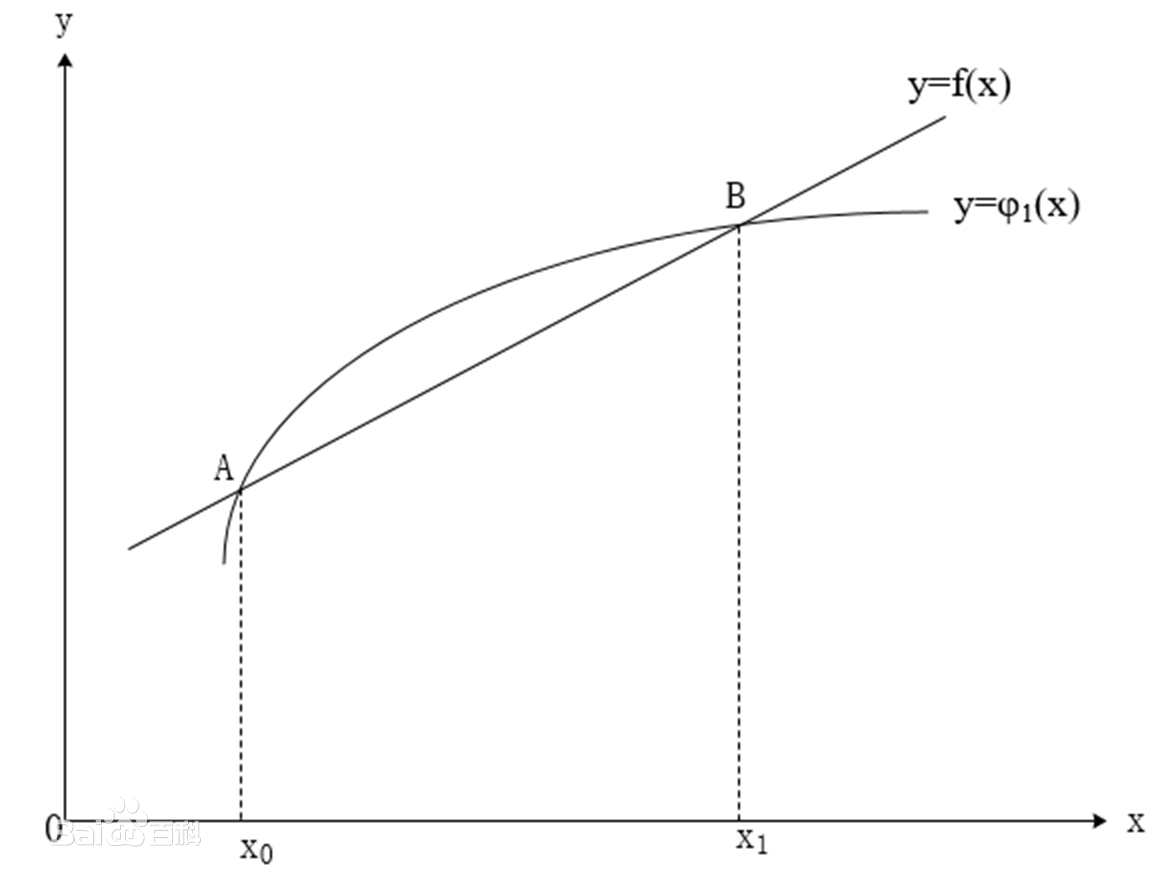
\includegraphics[width=.7\textwidth]{figures//fig3-2.png}
	\caption{线性插值示意图}
	\label{fig3-2}
\end{figure}

如图\ref{fig3-2}所示,设函数$\rm y = f(x)$在$\rm x_0$,$\rm x_1$点的取值分别为$\rm y_0$,$\rm y_1$,求多项式
$$\rm y = φ_1(x) = a_0+a_1x$$
使满足
$$\rm φ_1(x_0) = y_0, φ_1(x1) = y_1 $$
由解析几何易得:
$$\rm y = φ_1(x) = y_0 +\frac{y_1-y_0}{x_1-x_0}(x-x_0)	$$
使用线性插值法可以填补表中的缺失值,并在之后的处理过程中将插入值作为缺失值的替代

(2)通过污染物浓度计算AQI指数:
AQI指数的计算方法在问题一中已经进行阐述,此处不再赘述。对每个小时的污染物浓度数据,都可以计算出其相应的AQI指数。

(3)数据的标准化:
由于数据的量纲不同,我们需要变量数据进行标准化。标准化原始变量数据采用如公式(3)方式:
\begin{equation}
	\rm ZX_i = \frac{X_i-μ}{δ}, μ = \frac{1}{n}\sum_{i=1}^{n}X_i, δ = \sqrt{\frac{1}{n-1}\sum_{i=1}^{n}(X_i-μ)^2}
\end{equation}
将标准化之后AQI,SO3,NO2,O3,PM10,PM2.5,CO变量对应的新变量分别命名为ZAQI,ZSO3,ZNO2,ZO3,ZPM10,ZPM2.5,ZCO。将标准化之后的T,H,P,WS,WD等变量分别命名为ZT,ZH,ZP,ZWS,ZWD

\subsubsection{模型建立、求解与验证}
(1)Person相关系数分析

在本题中,研究变量之间的相关性采用Pearson相关系数进行分析。Pearson相关系数是用来衡量两个数据集合是否在一条线上面,它用来衡量定距变量间的线性关系的一种评价指标。当两个变量都是正态连续变量,而且两者之间呈线性关系时,表现这两个变量之间相关程度用积差相关系数,主要有Pearson简单相关系数。
其计算方式如公式(4)所示:
\begin{equation}
	\rm r = \frac{N\sum{x_iy_i}-\sum{x_i}\sum{y_i}}{\sqrt{N\sum{x_i^2}-(\sum{x_i})^2}\sqrt{N\sum{y_i^2}-(\sum{y_i})^2}}
\end{equation}
Pearson相关系数衡量的是线性相关关系。若r=0,只能说x与y之间无线性相关关系,不能说无相关关系。相关系数的绝对值越大,相关性越强:相关系数越接近于1或-1,相关度越强,相关系数越接近于0,相关度越弱。
此处使用Python和SPSS统计软件,分析ZAQI,ZNO2,ZSO3,ZO3,ZCO,ZPM10,ZPM2.5之间的Person相关性的步骤如下:
\ding{172} 使用Python对Excel数据进行处理,通过线性插值填补缺失值,并计算出每一行对应的AQI指数

\ding{173} 使用SPSS软件导入Excel数据

\ding{174} 通过SPSS软件,点击分析→描述统计→描述,选择AQI等12个变量,并将标准化之后的变量另存为变量ZAQI等变量。

\ding{175} 通过SPSS软件,点击相关→双变量,选择ZAQI、ZCO等6个变量,得到其Pearson相关系数矩阵

其相关系数矩阵如图\ref{fig3-3}所示:
\begin{figure}[!h]
	\centering
	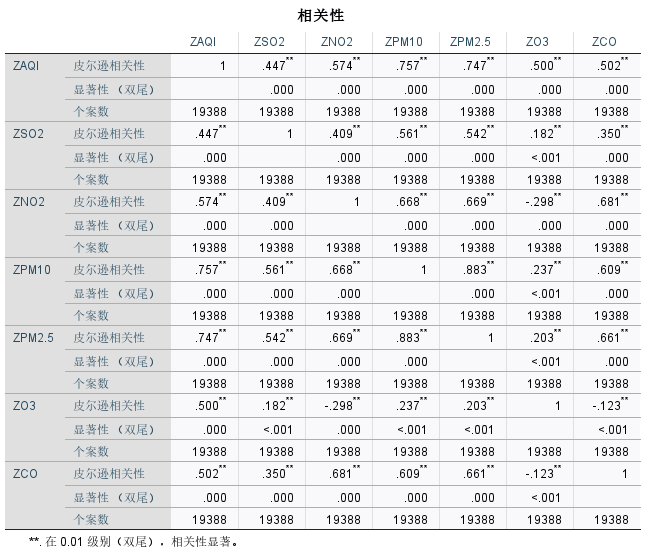
\includegraphics[width=.7\textwidth]{figures//fig3-3.png}
	\caption{ZAQI变量Person相关矩阵示意图}
	\label{fig3-3}
\end{figure}

(2)通过Critic赋权法和主观调整确定AP表达式

确定某种变量的权重主要有两大类:一类是主观权重赋值法,例如AHP、专家评分法等;还有一类就是客观权重赋权法,比较典型的就是Critic赋值法。
Critic赋值法以两个基本概念为基础:一是对比强度,借鉴标准离差法的思想,认为若同一指标的所有评价指数差别越大,即标准差越大,则所蕴含的信息量越大;二是评价指标之间的冲突性,指标之间的冲突性是以指标之间的相关系数为基础,如两个指标之间具有较强的正相关,说明两个指标冲突性较低。第j个指标与其它指标的冲突性的量化指标$\rm \sum_{i=1}^{n}(1-r_{ij})$,其中$\rm r_{ij}$评价指标i和j之间的相关系数。各个指标的客观权重确定就是以对比强度和冲突性来综合衡量的。设$\rm C_j$表示第j个评价指标所包告的信息量。$\rm C_j$的计算式如下:
$$
\rm C_j=δ_j \sum_{i=1}^{n}1-r_{ij}     
$$
其中n为同一指标的评价数量。一般地,$\rm C_j$越大,第j个评价指标所包含的信息量越大,则该指标的相对重要性也就越大。

设$\rm W_j$为第j个指标的客观权重。$\rm W_j$的计算公式:$\rm W_j=\frac{C_j}{\sum_{i=1}^{m}C_i} $(m为所有指标的数量)
通过Critic赋权法可以计算出对于自定义因变量AP关于ZNO2等变量的权重,最后通过加权求和的方式得到最终的计算公式:
\begin{equation}
	\rm AP = \sum_{i=1}^{n}W_iZX_i
\end{equation}
该过程的数学解释为:通过计算AQI与6中污染物的相关性,反映了不同的污染物,其浓度变化对AQI变化的影响,对AQI变化影响较大的污染物,赋予更高的权重。
通过Python程序,计算出的权重表如表\ref{tab:table4-4}所示:(精确至小数点后三位)
\begin{table}[h!]
	\caption{AP权重计算结果表}\label{tab:table4-4}
	\begin{center}
		\begin{tabular}{|c|c|c|c|c|c|}
			\hline
			变量名&权重&变量名&权重&变量名&权重 \\
			\hline
			ZSO2&0.127&ZNO2&0.163&ZPM10&0.215 \\
			\hline
			ZPM2.5&0.212&ZO3&0.142&ZCO& 0.142\\
			\hline
		\end{tabular}
	\end{center}
\end{table}

但是主观上认为直接使用该权重有一定的误差,因为在对监测点A逐小时污染数据处理计算AQI值和首要污染物之后,发现污染物CO和SO2成为首要污染物的比例非常低,甚至没有任何一个小时其SO2污染物为首要污染物。通过引入各个污染物成为首要污染物的比例,来修正各个变量的权重值。使用如下计算方式:
\begin{equation*}
	\rm newW_i = 0.6*W_i+0.4*P_i       P_i = \frac{T_i}{\sum{T_i}}
\end{equation*}
其中$\rm T_i$表示第i中污染物成为首要污染物的次数

进行修正之后得到的权重表如表\ref{tab:table4-5}所示:
\begin{table}[h!]
	\caption{AP权重计算结果表}\label{tab:table4-5}
	\begin{center}
		\begin{tabular}{|c|c|c|c|c|c|}
			\hline
			变量名&权重&变量名&权重&变量名&权重 \\
			\hline
			ZSO2&0.076&ZNO2&0.260&ZPM10&0.226 \\
			\hline
			ZPM2.5&0.165&ZO3&0.182&ZCO&0.091\\
			\hline
		\end{tabular}
	\end{center}
\end{table}

则有AP计算公式如下所示
\begin{equation*}
	\rm AP = 0.076*ZSO_2+0.260*ZNO_2+0.226*ZPM_{10}+0.165*ZPM_{2.5}+0.182*ZO_3+0.091*ZCO
\end{equation*}

(3)分析AP与气象条件因素的相关性并统计AP在某种气象条件下的平均值变化率
	通过SPSS软件直接定义新变量AP,通过定义计算表达式计算出AP的取值。然后对变量AP,GT,GH,GP,GWS,GWD等变量进行相关性分析,得到相关性矩阵如图\ref{fig3-4}所示:
	\begin{figure}[!h]
		\centering
		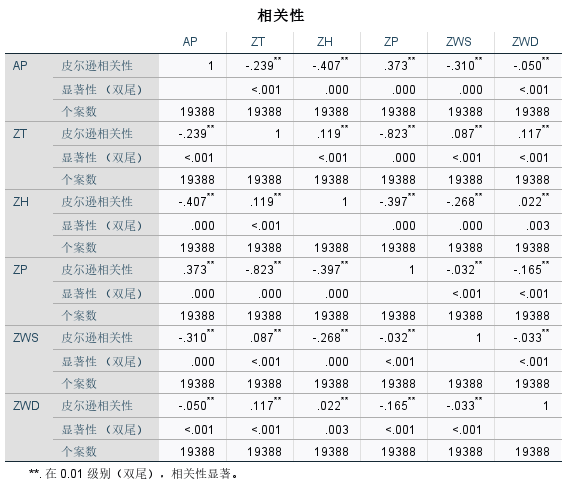
\includegraphics[width=.7\textwidth]{figures//fig3-4.png}
		\caption{变量AP的Person相关系数矩阵}
		\label{fig3-4}
	\end{figure}
	
	从图\ref{fig3-4}中各个变量对应的Pearson相关系数,我们可以看出:变量ZWD(即标准化之后的风速变量)对AP变量的影响比较小,其余因素对变量AP的取值都有较大影响,可视化统计AP变量与各个气象因素条件如下:
	
	\ding{172} 可视化统计AP变量与风速变量WS之间的关系:
	将“监测点A逐小时污染物浓度与气象实测数据”表中每小时风速变量WS与对应计算出的AP变量值进行一一对应,并求出每一个特定的WS取值下对应AP变量取值的均值。并将结果绘制为折线图,其结果如图\ref{fig3-5}所示:
	\begin{figure}[!h]
		\centering
		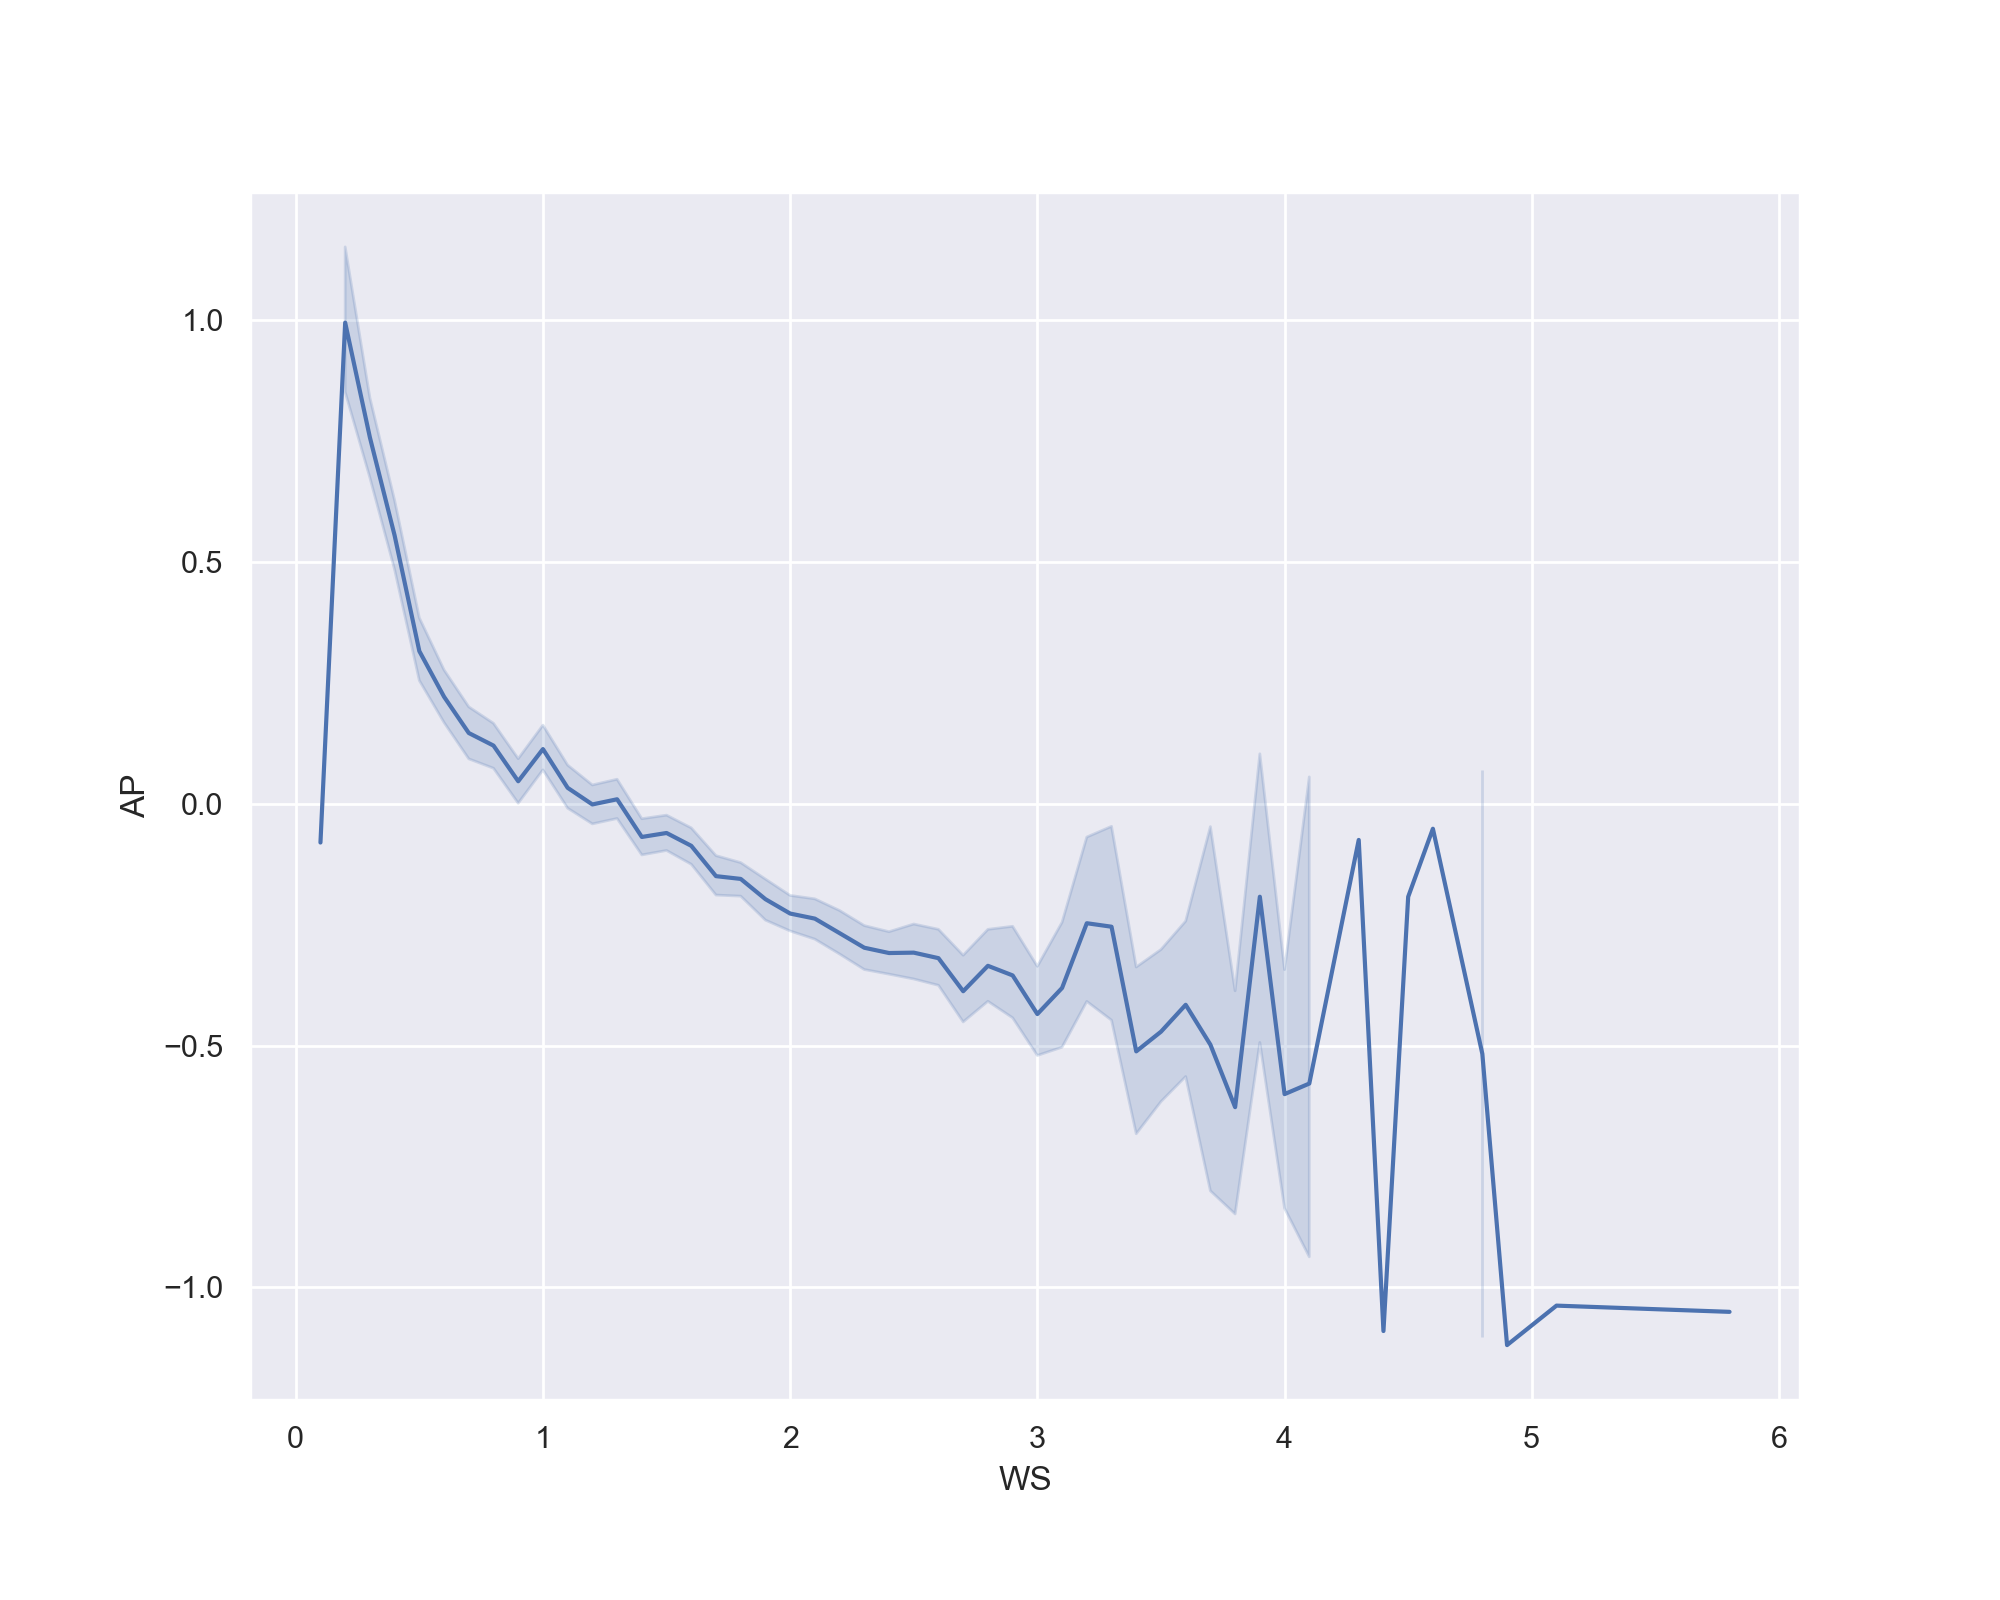
\includegraphics[width=.7\textwidth]{figures//fig_WS.png}
		\caption{变量AP的Person相关系数矩阵}
		\label{fig3-5}
	\end{figure}

虽然图中折线的震荡性非常强,
(4)将原始污染浓度数据可视化进行模型的验证
	不使用AP变量,直接使用
\subsection{问题三 依据一次预报数据和实测数据进行气象二次预报}
\subsubsection{问题描述和分析}
问题的分析问题的分析问题的分析问题的分析问题的分析问题的分析问题的分析问题的分析问题的分析问题的分析问题的分析问题的分析问题的分析问题的分析。
\subsubsection{模型建立与求解}
模型建立与求解模型建立与求解模型建立与求解模型建立与求解模型建立与求解模型建立与求解模型建立与求解模型建立与求解模型建立与求解模型建立与求解模型建立与求解。

\subsection{问题四 xxx}
\subsubsection{问题描述和分析}
问题的分析问题的分析问题的分析问题的分析问题的分析问题的分析问题的分析问题的分析问题的分析问题的分析问题的分析问题的分析问题的分析问题的分析。
\subsubsection{模型建立与求解}
模型建立与求解模型建立与求解模型建立与求解模型建立与求解模型建立与求解模型建立与求解模型建立与求解模型建立与求解模型建立与求解模型建立与求解模型建立与求解。

\section{模型的评价}
\subsection{模型的优点}
模型的优点模型的优点模型的优点模型的优点模型的优点模型的优点模型的优点模型的优点模型的优点模型的优点模型的优点模型的优点模型的优点模型的优点。
\subsection{模型的缺点}
模型的缺点模型的缺点模型的缺点模型的缺点模型的缺点模型的缺点模型的缺点模型的缺点模型的缺点模型的缺点模型的缺点模型的缺点模型的缺点模型的缺点。



\section{写作参考格式}
写作过程中可能要用到一些格式参考,正式写作的时候,可以直接将这一章删掉即可。

\textbf{无序列表格式}
\begin{itemize}
\item 无序列表1
\item 无序列表2
\item 无序列表3
\item 无序列表4
\end{itemize}


\textbf{表格格式}

\begin{tabular}{cc}
 \hline
 \makebox[0.4\textwidth][c]{符号}	&  \makebox[0.5\textwidth][c]{意义} \\ \hline
 D	    & 宽度(cm) \\ \hline
 L	    & 长度(cm)  \\ \hline
\end{tabular}


%
%\textbf{图片格式}
%\begin{figure}[h]
%\centering
%\includegraphics[width=5cm]{xxx.jpg}
%\caption{图片标题}
%\end{figure}

\section{参考文献}
%参考文献
\begin{thebibliography}{1.2}%宽度9
\setlength{\itemsep}{-2mm}
 \bibitem{ref1}
 宋鹏程, 张馨文, 黄强, 等. 我国城市环境空气质量预报主要模型及应用[J]. 四川环境, 2019, 3.
 \bibitem{ref2}
 伯鑫 等. 空气质量模型(SMOKE、WRF、CMAQ等)操作指南及案例研究 [M]. 北京: 中国环境出版集团, 2019.
 \bibitem{ref3}
 戴树桂. 环境化学 [M]. 北京: 高等教育出版社, 1997.
 \bibitem{ref4}
 赵秋月, 李荔, 李慧鹏. 国内外近地面臭氧污染研究进展 [J]. 环境科技, 2018, 31(05): 72-76.
 \bibitem{ref5}
 陈敏东. 大气臭氧污染形成机制及研究进展 [J/OL] 2018, https://max.book118.com/html/2018/0201/151478594.shtm. 
\end{thebibliography}

\newpage
%附录
\appendix
\section{程序代码}
%设置不同语言即可。
\begin{lstlisting}[language=Matlab] 
kk=2;[mdd,ndd]=size(dd);
while ~isempty(V)
[tmpd,j]=min(W(i,V));tmpj=V(j);
for k=2:ndd
[tmp1,jj]=min(dd(1,k)+W(dd(2,k),V));
tmp2=V(jj);tt(k-1,:)=[tmp1,tmp2,jj];
end
tmp=[tmpd,tmpj,j;tt];[tmp3,tmp4]=min(tmp(:,1));
if tmp3==tmpd, ss(1:2,kk)=[i;tmp(tmp4,2)];
else,tmp5=find(ss(:,tmp4)~=0);tmp6=length(tmp5);
if dd(2,tmp4)==ss(tmp6,tmp4)
ss(1:tmp6+1,kk)=[ss(tmp5,tmp4);tmp(tmp4,2)];
else, ss(1:3,kk)=[i;dd(2,tmp4);tmp(tmp4,2)];
end;end
dd=[dd,[tmp3;tmp(tmp4,2)]];V(tmp(tmp4,3))=[];
[mdd,ndd]=size(dd);kk=kk+1;
end; S=ss; D=dd(1,:);
 \end{lstlisting}


\end{document} 